\documentclass{myhw}
\linespread{1.05}        % Palatino needs more leading (space between lines)
\usepackage{extarrows}
\usepackage{mathrsfs}
\usepackage{braket}
\titleformat{\section}[runin]{\sffamily\bfseries}{}{}{}[]
\titleformat{\subsection}[runin]{\sffamily\bfseries}{}{}{}[]
\renewcommand{\exname}{Question }
\renewcommand{\subexcounter}{(\alph{homeworkSectionCounter})}
\newcommand{\id}{\text{Id}}
\newcommand{\tr}{\text{Tr}}
\newcommand{\rib}{\text{Rib}}

\title{CSC 2515 Homework 2}
\begin{document}

%% Question 1
\begin{homeworkProblem}
\textbf{Robust Regression.}
%%% Subquestion 1
\begin{homeworkSection}
Sketch the Huber loss $L_\delta(y,t)$ and squared error loss $L_{SE}(y,t) = \frac{1}{2}(y - t)^2$ for $t = 0$, either by hand or using a plotting library. Based on your sketch, why would you expect the Huber loss to be more robust to outliers? \\
\\
When $t=2$, 
\begin{gather*}
L_{SE}(y,t) = \frac{1}{2}(y - t)^2 = \frac{1}{2}y^2 \\
L_\delta(y,t) = H_\delta(y-t) = \left\{ 
	\begin{array}{lr} 
	\frac{1}{2}y^2 & if\ |a| \le \delta \\ 
	\delta \times (|y|-\frac{1}{2}\delta) & if\ |a| > \delta
	\end{array} \right.
\end{gather*}
With the help of matplotlib, their sketches are shown in Figure \ref{fig:q1.1}. 
\begin{figure}[h]
  \centering
  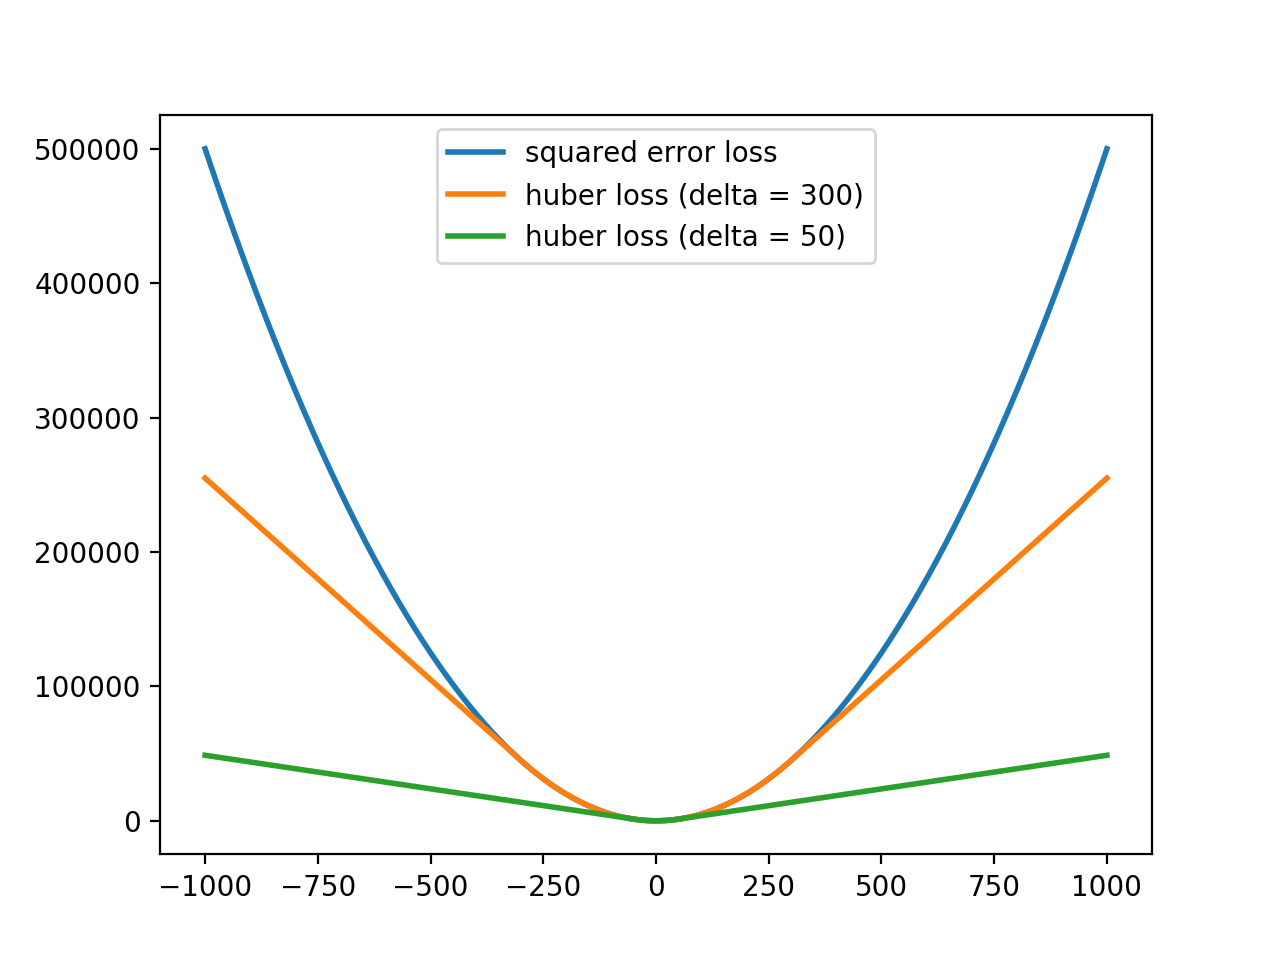
\includegraphics[width=.7\textwidth]{q1.png} 
  \caption{Sketches of squared error loss and Huber loss function. }
  \label{fig:q1.1}
\end{figure}
\\
As you can see from the Figure \ref{fig:q1.1}, for LSE functions, when the value $|y|$ is large (which is also the case with outliers), $L_{SE}(y,t)$ is very sensitive to $|y|$ (and outliers). 
On the contrary, for Huber loss function, when $|y|$ exceeds $\delta$, $L_\delta(y, t)$ increases linearly to $|y|$, which shows that it is relatively less sensitive to outliers.
\end{homeworkSection}
%%% Subquestion 2
\begin{homeworkSection}
%Just as with linear regression, assume a linear model: $y=\textbf{w}^T\textbf{x}+b$.
Give formulas for the partial derivatives $\partial L_\delta / \partial \textbf{w}$ and $\partial L_\delta / \partial b$. \\
\\
The formula for the derivative $H_\delta '(a)$ is
\begin{gather*}
H_\delta'(a) = 
	\left\{ 
	\begin{array}{lr} 
	a & if\ |a| \le \delta \\ 
	\delta & if\ a > \delta \\
	- \delta & if\ a < -\delta
	\end{array} \right.
\end{gather*}
Then, in terms of $a=y-t$, 
\begin{gather*}
H_\delta'(y-t) = 
	\left\{ 
	\begin{array}{lr} 
	y-t & if\ |y-t| \le \delta \\ 
	\delta & if\ y > t + \delta \\
	- \delta & if\ y < t - \delta
	\end{array} \right.
\end{gather*}
As for the linear model, \\if $\textbf{x}$ and $\textbf{w}$ are both $D$ dimensional vectors. 
\begin{gather*}
y = \textbf{w}^T\textbf{x} + b = \sum_j{w_j x_j + b} \\
\begin{aligned}
H_\delta'(y-t) = \frac{\partial H_\delta}{\partial y} & = 
	\left\{ 
	\begin{array}{lr} 
	\sum_j{w_j x_j + b} - t & if\ |y-t| \le \delta \\ 
	\delta & if\ y > t + \delta \\
	- \delta & if\ y < t - \delta
	\end{array} \right.
\\
\frac{\partial L_\delta}{\partial w_j} = \frac{\partial H_\delta}{\partial w_j} = 
\frac{\partial H_\delta}{\partial y} \frac{\partial y}{\partial w_j} & = 
	\left\{ 
	\begin{array}{lr} 
	x_j (\sum_{j'}{w_{j'} x_{j'} + b} - t) & if\ |y-t| \le \delta \\ 
	\delta x_j & if\ y > t + \delta \\
	- \delta x_j & if\ y < t - \delta
	\end{array} \right.
\\
\frac{\partial L_\delta}{\partial b} = \frac{\partial H_\delta}{\partial b} =
\frac{\partial H_\delta}{\partial y^{(i)}} \frac{\partial y^{(i)}}{\partial b} & = 
	\left\{ 
	\begin{array}{lr} 
	\sum_{j}{w_{j} x_{j} + b - t} & if\ |y-t| \le \delta \\ 
	\delta & if\ y > t + \delta \\
	- \delta & if\ y < t - \delta
	\end{array} \right.
\\
\frac{\partial L_\delta}{\partial \textbf{w}} & = 
	\left\{ 
	\begin{array}{lr} 
	\textbf{x}(\textbf{x}^T\textbf{w} + b - t) & if\ |y-t| \le \delta \\ 
	\delta \textbf{x} & if\ y > t + \delta \\
	- \delta \textbf{x} & if\ y < t - \delta
	\end{array} \right.
\\
\end{aligned}
\end{gather*}
When $\textbf{X}$ is a $N \times D$ matrix and $\textbf{w}$ is a $D$ dimensional vector. 
Then, 
\begin{gather*}
\textbf{y}=\textbf{X}\textbf{w}+b\textbf{1}, \\ y^{(i)} = \sum_j{w_j x_j^{(i)} + b}
\end{gather*}
We define $\mathscr{E}$ as the model's cost function.
\begin{gather*}
\mathscr{E}_\delta = \frac{1}{N}\sum_{i=1}^N{L_\delta} = \frac{1}{N}\sum_{i=1}^N{H_\delta}
\end{gather*}
We apply $y^{(i)}$ in the partial derivatives, 
\begin{gather*}
\begin{aligned}
\frac{\partial H_\delta}{\partial y^{(i)}} & = 
	\left\{ 
	\begin{array}{lr} 
	\sum_j{w_j x_j^{(i)} + b} - t^{(i)} & if\ |y^{(i)}-t^{(i)}| \le \delta \\ 
	\delta & if\ y^{(i)} > t^{(i)} + \delta \\
	- \delta & if\ y^{(i)} < t^{(i)} - \delta
	\end{array} \right.
\\
\frac{\partial \mathscr{E}_\delta}{\partial w_j} = 
\frac{\partial \mathscr{E}_\delta}{\partial y^{(i)}} \frac{\partial y^{(i)}}{\partial w_j} & = 
	\frac{1}{N} \sum_{i=1}^N
	\left\{ 
	\begin{array}{lr} 
	{x_j^{(i)} (\sum_{j'}{w_{j'} x_{j'}^{(i)} + b} - t^{(i)})} & if\ |y^{(i)}-t^{(i)}| \le \delta \\ 
	{\delta x_j^{(i)}} & if\ y^{(i)} > t^{(i)} + \delta \\
	- {\delta x_j^{(i)}} & if\ y^{(i)} < t^{(i)} - \delta
	\end{array} \right.
\\
\frac{\partial \mathscr{E}_\delta}{\partial b} = 
\frac{\partial \mathscr{E}_\delta}{\partial y^{(i)}} \frac{\partial y^{(i)}}{\partial b} & = 
	\frac{1}{N} \sum_{i=1}^N
	\left\{ 
	\begin{array}{lr} 
	(\sum_{j}{w_{j} x_{j}^{(i)} + b} - t^{(i)}) & if\ |y^{(i)}-t^{(i)}| \le \delta \\ 
	\delta & if\ y^{(i)} > t^{(i)} + \delta \\
	- \delta & if\ y^{(i)} < t^{(i)} - \delta
	\end{array} \right.
\end{aligned}
\end{gather*}
The partial derivatives can also be represented by matrix-vector format, 
\begin{gather*}
\begin{aligned}
\frac{\partial \mathscr{E}_\delta}{\partial \textbf{w}} & = 
	\left\{ 
	\begin{array}{lr} 
	\frac{1}{N} \textbf{X}^T(\textbf{Xw} + b\textbf{1} - \textbf{t}) & if\ - \delta \textbf{1} \le \textbf{y}-\textbf{t} \le \delta \textbf{1} \\ 
	\frac{\delta}{N} \textbf{X}^T \textbf{1} & if\ \textbf{y} > \textbf{t} + \delta \textbf{1} \\
	- \frac{\delta}{N} \textbf{X}^T \textbf{1} & if\ \textbf{y} < \textbf{t} - \delta \textbf{1}
	\end{array} \right.
\end{aligned}
\end{gather*}
\end{homeworkSection}
%%% Subquestion 3
\begin{homeworkSection}
Write Python code to perform (full batch mode) gradient descent on this model. \\
\\
The update rule of gradient descent method is as follows, 
\begin{gather*}
w_j \leftarrow w_j - \alpha \frac{\partial \mathscr{E}_\delta}{\partial w_j} \\
\textbf{w} \leftarrow \textbf{w} - \alpha \frac{\partial \mathscr{E}_\delta}{\partial \textbf{w}} 
\end{gather*}
Without using \textbf{for} loop, we applied the \textbf{np.where} function to realize the gradient descent on the Huber loss function. 
First, we generalized three vectors using $\textbf{y}-\textbf{t}$, $\delta \textbf{1}$ and $-\delta \textbf{1}$ separately; 
then we used \textbf{np.where} to determine which line of the three vectors should be chosen.
\\
I sampled 50000 samples through $y=3x_1 + 5x_2 - 9x_3 + 28x_4 -10x_5 + 0$. Through 1000 iterations, the loss dropped to 0.01384. The predicted w was $[3.000181, 5.00041, -9.00045, 28.000627, -10.000461, 0.000123]$. However, I evaluated the efficiency of the algorithms with Huber loss function or square error loss function, and found that they took 6.6 and 0.24 seconds, respectively. I guessed the \textbf{np.where} function takes up most of the total time.
\\
\\
Code is in q1.py.
\end{homeworkSection}
\end{homeworkProblem}


%% Question 2
\begin{homeworkProblem}
\textbf{Locally Weighted Regression.}
%%% Subquestion 1
\begin{homeworkSection}
Show the solution to the weighted least squares problem. \\
\\
We define $\mathscr{E}$ as the function of the weighted least squares problem.
\begin{gather*}
\mathscr{E} = \frac{1}{2} \sum_{i=1}^N{a^{(i)} (y^{(i)} - \textbf{w}^T \textbf{x}^{(i)})^2} + \frac{\lambda}{2} ||\textbf{w}||^2
\end{gather*}
To get solution for the problem, $\textbf{w}^*$, we need partial derivatives to zero.
\begin{gather*}
\begin{aligned}
\frac{\partial \mathscr{E}}{\partial w_j} = \sum_{i=1}^N{a^{(i)} (y^{(i)} - \textbf{w}^T \textbf{x}^{(i)})x_j^{(i)}} + \lambda w_j & = 0 \\
\sum_{i=1}^N{a^{(i)} y^{(i)} x_j^{(i)}} - \sum_{i=1}^N{a^{(i)} x_j^{(i)} \textbf{w}^T \textbf{x}^{(i)}} + \lambda w_j & = 0 \\
\sum_{i=1}^N{a^{(i)} x_j^{(i)} \textbf{w}^T \textbf{x}^{(i)}} - \lambda w_j & = \sum_{i=1}^N{a^{(i)} y^{(i)} x_j^{(i)}} \\
\textbf{X}^T \textbf{AXw} - \lambda \textbf{1w} & = \textbf{X}^T \textbf{Ay} \\
\textbf{w} & = (\textbf{X}^T \textbf{AX} - \lambda \textbf{1})^{-1} \textbf{X}^T \textbf{Ay}
\end{aligned}
\end{gather*}
\end{homeworkSection}
%%% Subquestion 2
\begin{homeworkSection}

\end{homeworkSection}
%%% Subquestion 3
\begin{homeworkSection}

\end{homeworkSection}
\end{homeworkProblem}


%% Question 3
\begin{homeworkProblem}
\textbf{AdaBoost.} \\
\\

\end{homeworkProblem}
\end{document}

%\begin{gather*}
%\end{gather*}

